\newcommand{\tmpwidth}{0.23\linewidth}
\setlength{\tabcolsep}{1pt}
\begin{figure}[!t]
    \centering
    \begin{tabular}{c c c c }

	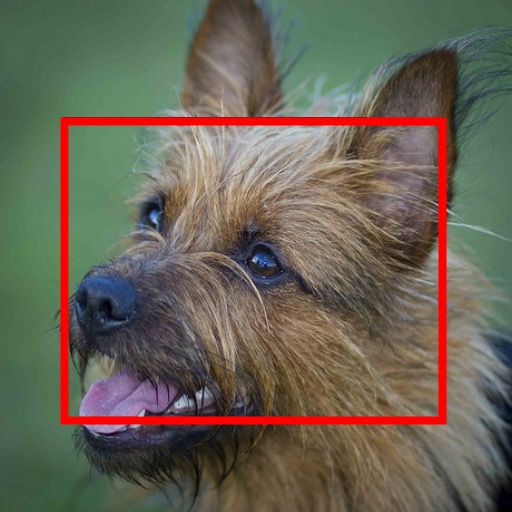
\includegraphics[width=\tmpwidth]{figures/editing/000193_to282_0006_input.jpeg} &
	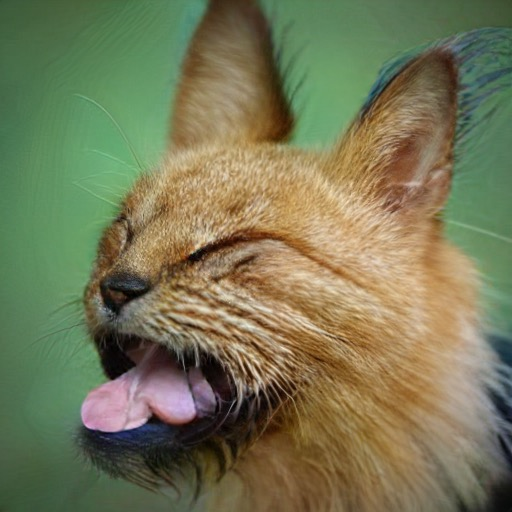
\includegraphics[width=\tmpwidth]{figures/editing/000193_to282_0006_output.jpeg}&
	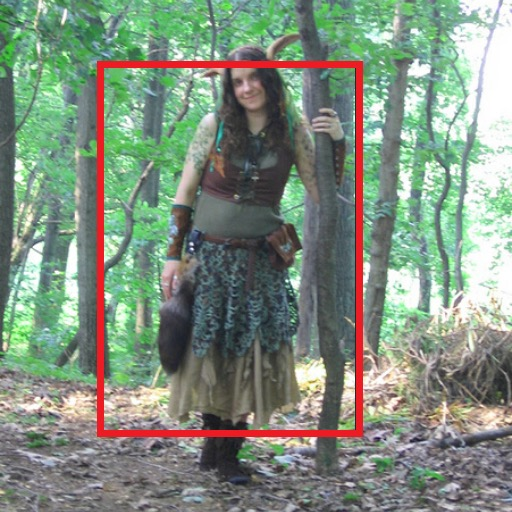
\includegraphics[width=\tmpwidth]{figures/editing/000689_to282_0000_input.jpeg} &
	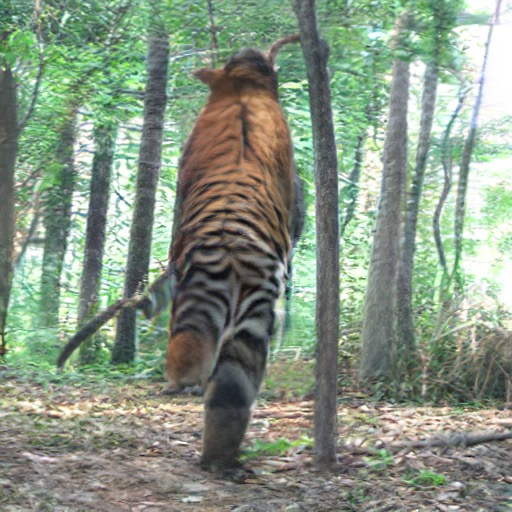
\includegraphics[width=\tmpwidth]{figures/editing/000689_to282_0000_output.jpeg} 
	\\
	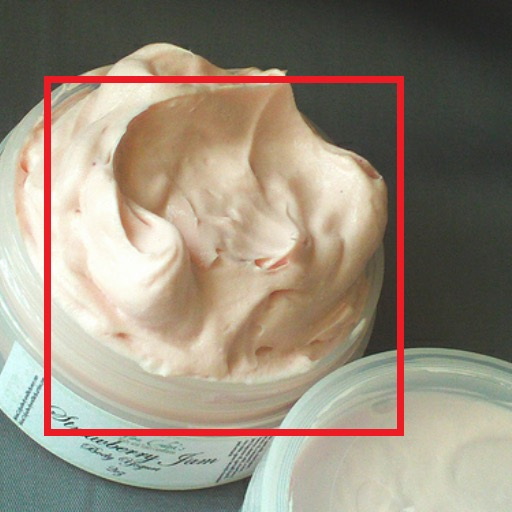
\includegraphics[width=\tmpwidth]{figures/editing/000838_to282_0004_input.jpeg} &
	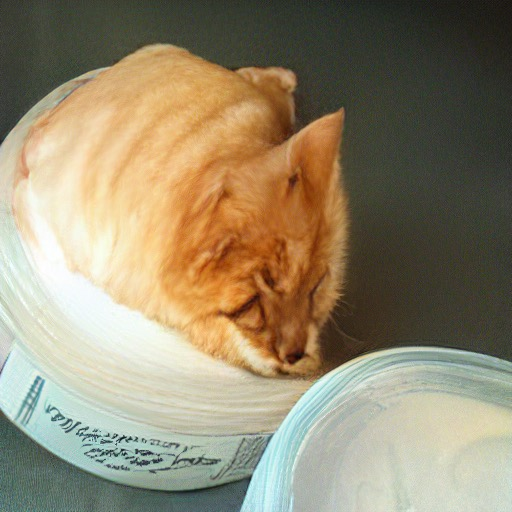
\includegraphics[width=\tmpwidth]{figures/editing/000838_to282_0004_output.jpeg} &
	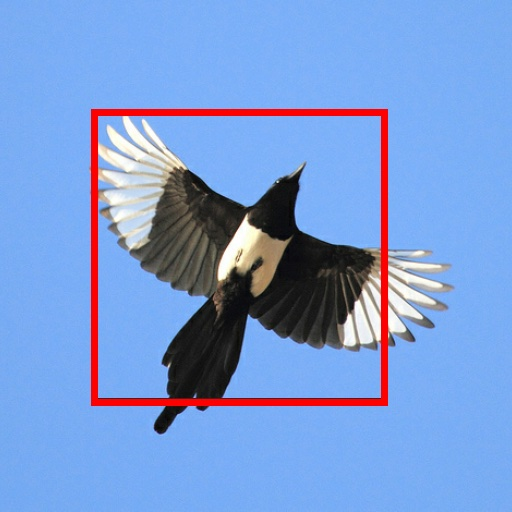
\includegraphics[width=\tmpwidth]{figures/editing/000018_to282_0002_input.jpeg} &
	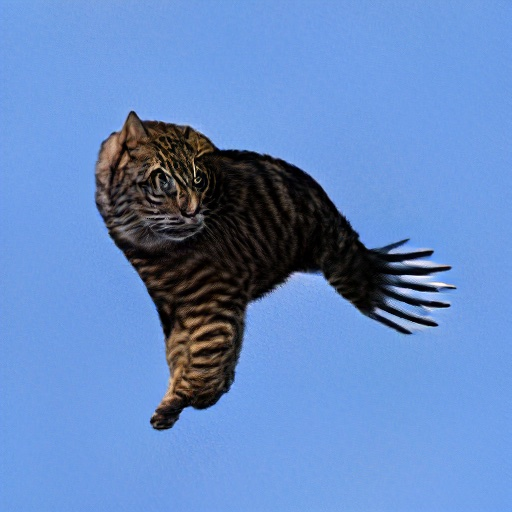
\includegraphics[width=\tmpwidth]{figures/editing/000018_to282_0000_output.jpeg} 
	
	\\
	
	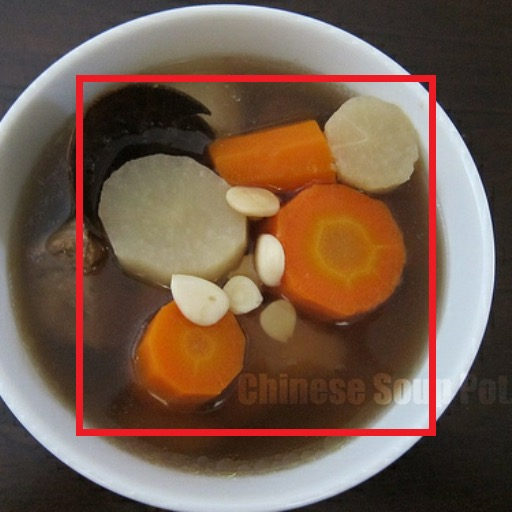
\includegraphics[width=\tmpwidth]{figures/editing/000809_to282_0002_input.jpeg} &
	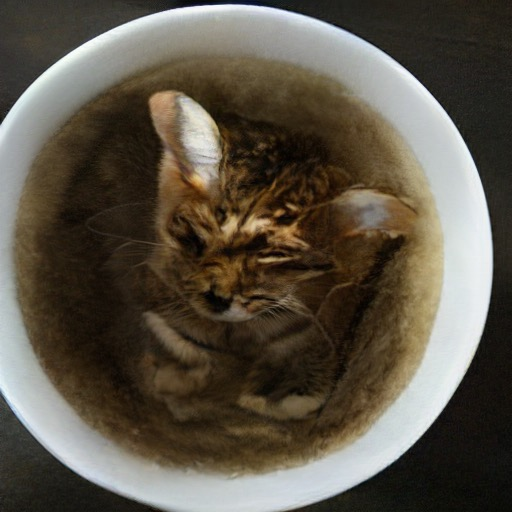
\includegraphics[width=\tmpwidth]{figures/editing/000809_to282_0002_output.jpeg} &
	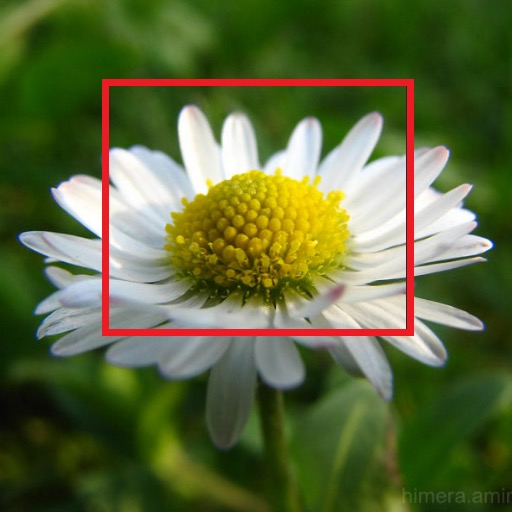
\includegraphics[width=\tmpwidth]{figures/editing/000985_to282_0000_0024_input.jpeg} &
    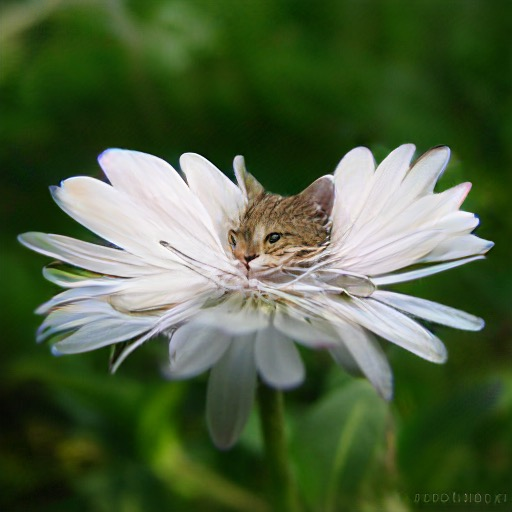
\includegraphics[width=\tmpwidth]{figures/editing/000985_to282_0000_0012_output.jpeg} 
    \\ 

    % \includegraphics[width=\tmpwidth]{figures/editing/000538_to282_0036_output.jpeg} &

    \end{tabular}
    \vspace{-3mm}
    \caption{\textbf{Class-conditional image editing.} Given input images on the left of each pair, and a target class "tiger cat", \model replaces the bounding boxed regions with tiger cats, suggesting the composition ability of our model. % The fact that the synthesized tiger cat blends in with the rest of the image seamlessly highlights the composition ability of our model. 
    }
    \vspace{-2mm}
    \label{fig:editing}
\end{figure}


\begin{figure}[!t]
    \centering
    \begin{tabular}{cccc}
  
    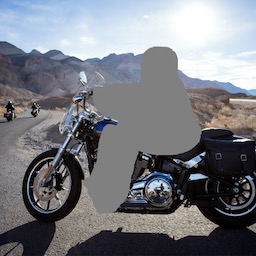
\includegraphics[width=\tmpwidth]{figures/uncrop/harley-davidson-xAHtaYIHlPI_input_0.jpeg}&

    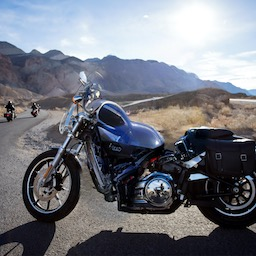
\includegraphics[width=\tmpwidth]{figures/uncrop/harley-davidson-xAHtaYIHlPI_output_12.jpeg}&
    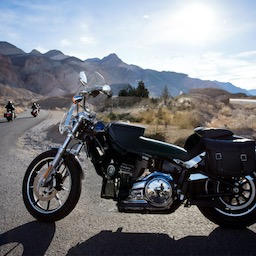
\includegraphics[width=\tmpwidth]{figures/uncrop/harley-davidson-xAHtaYIHlPI_output_03.jpeg}&
    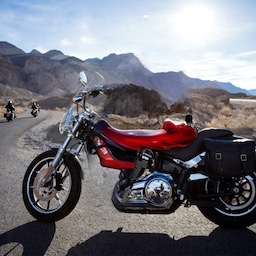
\includegraphics[width=\tmpwidth]{figures/uncrop/harley-davidson-xAHtaYIHlPI_output_06__.jpeg}

    \\
    
    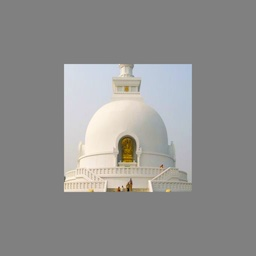
\includegraphics[width=\tmpwidth]{figures/uncrop/001704_input.jpeg}&
    % 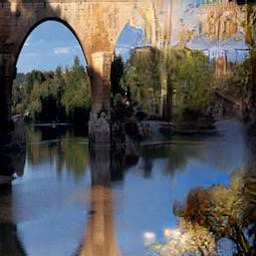
\includegraphics[width=\tmpwidth]{figures/uncrop/3101_boundless.jpeg}&
    % 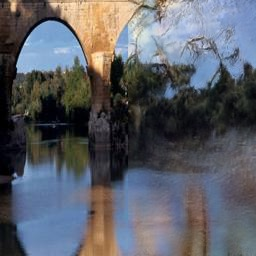
\includegraphics[width=\tmpwidth]{figures/uncrop/3101_inf.jpeg}&
    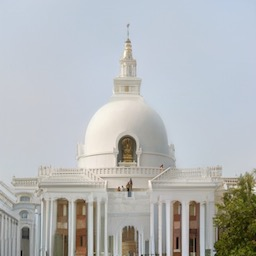
\includegraphics[width=\tmpwidth]{figures/uncrop/001704_ours_12.jpeg} &
    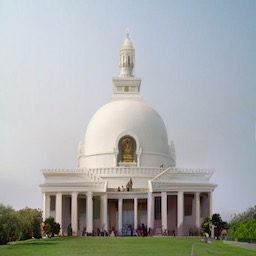
\includegraphics[width=\tmpwidth]{figures/uncrop/001704_ours_17.jpeg} &
    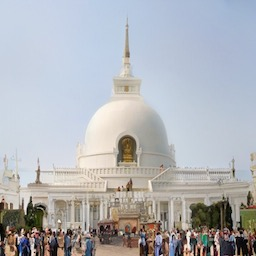
\includegraphics[width=\tmpwidth]{figures/uncrop/001704_ours_11.jpeg} 
    
    \\
    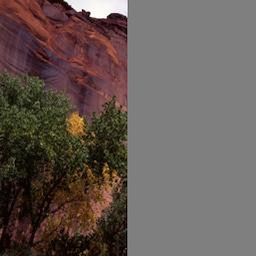
\includegraphics[width=\tmpwidth]{figures/uncrop/3996_input.jpeg}&
    %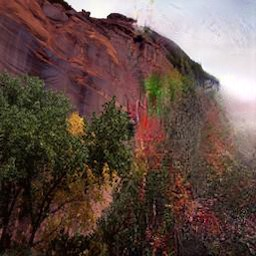
\includegraphics[width=\tmpwidth]{figures/uncrop/3996_boundless.jpeg}&
    % 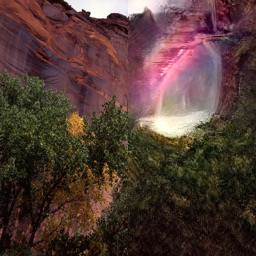
\includegraphics[width=\tmpwidth]{figures/uncrop/3996_inf.jpeg}&
    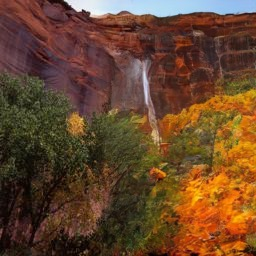
\includegraphics[width=\tmpwidth]{figures/uncrop/3996_output8.jpeg} &
    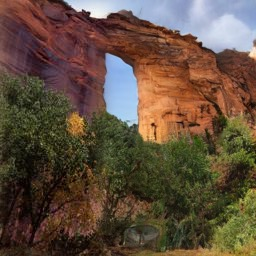
\includegraphics[width=\tmpwidth]{figures/uncrop/3996_output1.jpeg} &
    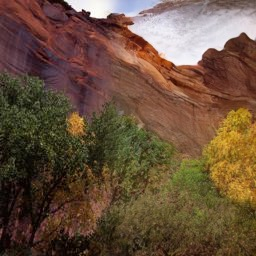
\includegraphics[width=\tmpwidth]{figures/uncrop/3996_output9.jpeg} 
    %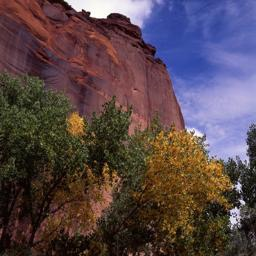
\includegraphics[width=\tmpwidth]{figures/uncrop/3996_gt.jpeg}
   \\
    \vspace{-1mm}
    Input  & \multicolumn{3}{c}{------ \model (Our Samples) ------} \\    
    % Input & DeepFill & HiFill  & \multicolumn{3}{c}{------ \model (Our Samples) ------} & Groundtruth \\    
    \end{tabular}
    \vspace{-1mm}
    \caption{\textbf{Inpainting and outpainting.} Given a single input image, \model synthesizes diverse results for inpainting (first row) and outpainting in different directions (last two rows).}
    \label{fig:uncrop_diversity}
    \vspace{-3mm}
\end{figure}

\setlength{\tabcolsep}{4pt}
\begin{table}[h]
\small
    \centering
    \resizebox{.92\linewidth}{!}{
    \begin{tabular}{llc ccc}
    \toprule
    {Task} & {Model} &
    & {FID}  $\downarrow$ & {IS} $\uparrow$ & %{L1} $\downarrow$ 
   % {Fool Rate} $\uparrow$ 
    \\
    \midrule
    \textit{\textbf{Outpainting}}
    & 
    Boundless \cite{teterwak2019boundless}$^{\square}$ & 
    & 35.02 & 6.15 & 
    %.064%
    \\
    % NS-Outpaint \cite{}$^{\square}$ &
    % & 50.68 & 4.70 &   \\   
     {\footnotesize Right 50\%} & In\&Out \cite{cheng2021inout}$^{\square}$ &
    & 23.57 & 7.18 &  \\
    & InfinityGAN \cite{lin2021infinitygan} &
    & 10.60 & 5.57 &
    \\
    & Boundless \cite{teterwak2019boundless} TF $^{\blackdiamond}$ & 
    & 7.80 & 5.99 &
    %.064% 
    \\
    %  & CoModGAN \cite{zhao2021comodgan}$^{512}$ &
    % & 7.67 & 9.09 &
    % %.064% 
    % \\
    & \textbf{\model (Ours)} $^{512}$& 
    & \textbf{6.78} & \textbf{11.69} &  \\ % [1pt]
    \midrule
    \textit{\textbf{Inpainting}} & 
     DeepFill \cite{yu2019free} &
    & 11.51 & 22.55 & \\
    {\footnotesize Center 50\%$\times$50\%} 
    & ICT\cite{wan2021ict}$^\dagger$ & 
    & 13.63 & 17.70 &  \\    
    & HiFill \cite{yi2020contextual}$^{512}$ & 
    & 16.60 & 19.93 &  \\
    & CoModGAN\cite{zhao2021comodgan}$^{512}$ &
    & \textbf{7.13} & 21.82 & \\    
    & \textbf{\model (Ours)$^{512}$} &
    & 7.92 & \textbf{22.95} & \\
    \bottomrule
    \end{tabular}
    }
\vspace{-2mm}
    \caption{\textbf{Quantitative Comparisons for Inpainting and Outpainting on Places2.} \footnotesize{$^{512}$ evaluated on 512$\times$512 samples while others evaluated on the corresponding 256$\times$256 ones, consistent with their training; $^\square$~taken from the prior work; $^\dagger$~evaluated using the released model trained on a subset of Places2; $^\blackdiamond$~evaluated using the TFHub model\cite{boundless_tfhub}.} }
    \label{tab:inpaint_uncrop}
    \vspace{-3mm}
\end{table}


